Passing through the fog barrier, you stumble into a dream-like scene. The hallway ahead is identical to the one in which you were previously interred... but missing in sections, as if you were failing to picture the place in its entirety. You stand amongst a vast panorama of overcast heavens and fog-choked earth: a flagstone island in the sky. A few emaciated corpses lay in soft repose around its wreckage.\\

A section of tile breaks loose, dropping to the mezzanine below with a loud crack.\\

The man from before appears as if summoned by the sound. At this distance, you can finally get a look as his face--and truth be told, you do find it familiar. This man has played some integral part in your life’s story.\\

“Our flotsam has washed ashore. And now we shall assess the salvage.”\\

The man turns his palms upwards, and a few of the corpses begin to stir.\\

\subsection*{Victory Condition}
Defeat Zealot Eóghainn

\subsection*{Doom Events}
\begin{itemize}
\item \textbf{Every Round After the First:} \emph{Eóghainn steps into the fog.} Roll 3D6. Calculate a hex coordinate (X,Y) from any two sums of these three dice, and place Zealot Eóghainn on that tile. The chosen location must be a free and valid hex. If no combination is valid, then re-roll. Remove all condition tokens (including Knockdown) from his enemy sheet before moving.
\end{itemize}

\begin{tcolorbox}
\textbf{Note:} For example, if the roll comes up: 1, 2, 3. The player might calculate 1,5; 4,2; 2,4; or 5,1. Any combination of dice is acceptable, but all three dice must be used.
\end{tcolorbox}

\pagebreak

\subsection*{Encounter Table}
\begin{tcolorbox}
\textbf{Roll:} 1D6
\begin{center}
\begin{tabular}{ L | L | L }
\multicolumn{1}{c|}{\textbf{1}} & 
\multicolumn{1}{c|}{\textbf{2}} & 
\multicolumn{1}{c}{\textbf{3}} \\
\emph{Occult Parable} &
\textbf{A:} \emph{Fevered Chanting}\newline \textbf{B:} \emph{Open-Palm Slap}\newline \textbf{C:} \emph{Secret Word} &
\textbf{A:} \emph{Open-Palm Slap}\newline \textbf{B:} \emph{Secret Word}\newline \textbf{C:} \emph{Occult Parable}\\
\hline
\multicolumn{1}{c|}{\textbf{4}} & 
\multicolumn{1}{c|}{\textbf{5}} & 
\multicolumn{1}{c}{\textbf{6}} \\
\textbf{A:} \emph{Open-Palm Slap}\newline \textbf{B:} \emph{Secret Word}\newline \textbf{C:} \emph{Occult Parable} &
\textbf{A:} \emph{Fevered Chanting}\newline \textbf{B:} \emph{Open-Palm Slap}\newline \textbf{C:} \emph{Secret Word} &
\emph{Occult Parable} \\
\end{tabular}
\end{center}
All Risen Prisoner enemies will Move towards the character and attempt \emph{Swipe} after Eóghainn’s Turn.\\
 
 \textbf{Note:} Zealot Eóghainn will not commit \emph{Fevered Chanting} if it is already in effect.
\end{tcolorbox}

\subsection*{Enemy Sheets}
\hrule
\ \\
{\large \textbf{Zealot Eóghainn}}\\\\
\begin{tabular}{s s s}
\textbf{HP:} 18 & \textbf{Move:} 0\\
\textbf{M.DEF:} 1 & \textbf{L.DEF:} 3 & \textbf{D.DEF:} 2 \\
\textbf{F.DEF:} 2 & \textbf{RES:} 1 \\
\end{tabular}\\

\emph{Intelligent:} This entity is human, or possesses a human-like intellect.\\

\emph{Unwavering Faith:} This entity ignores the Stunned, Charmed, Maddened, and Fear conditions.\\

\emph{Alert:} This entity is immune to Backstab.\\

\textbf{Attacks:}
\begin{itemize}
\item \emph{Open-Palm Slap} - Inflict \emph{Unparryable} Stun on an adjacent entity.
\item \emph{Secret Word} - Deal 2 Smite ranged damage to an entity within 2-3 tiles.
\item \emph{Fevered Chanting} - Add 1 Enhanced Defense: \textbf{P.DEF} (3) condition token to this enemy sheet.
\item \emph{Occult Parable} - Roll 3D6. Create a hex coordinate (X,Y) from any two sums of these three dice, and place a Risen Prisoner on that tile. If no combination is valid, then re-roll.
\end{itemize}
\hrule
\ \\
{\large \textbf{Risen Prisoner}}\\\\
\begin{tabular}{s s s}
\textbf{HP:} 4 & \textbf{Move:} 2\\
\end{tabular}\\

\emph{Undead:} This entity ignores Bleed and Dark damage, and the Bleeding, Stunned, Charmed, Maddened, and Fear conditions.\\

\textbf{Attack:}
\begin{itemize}
\item \emph{Swipe} - Deal 2 \emph{Unparryable} Crush damage to an adjacent entity.
\end{itemize}

\pagebreak

\subsection*{Encounter Map}
\begin{center}
\framebox{
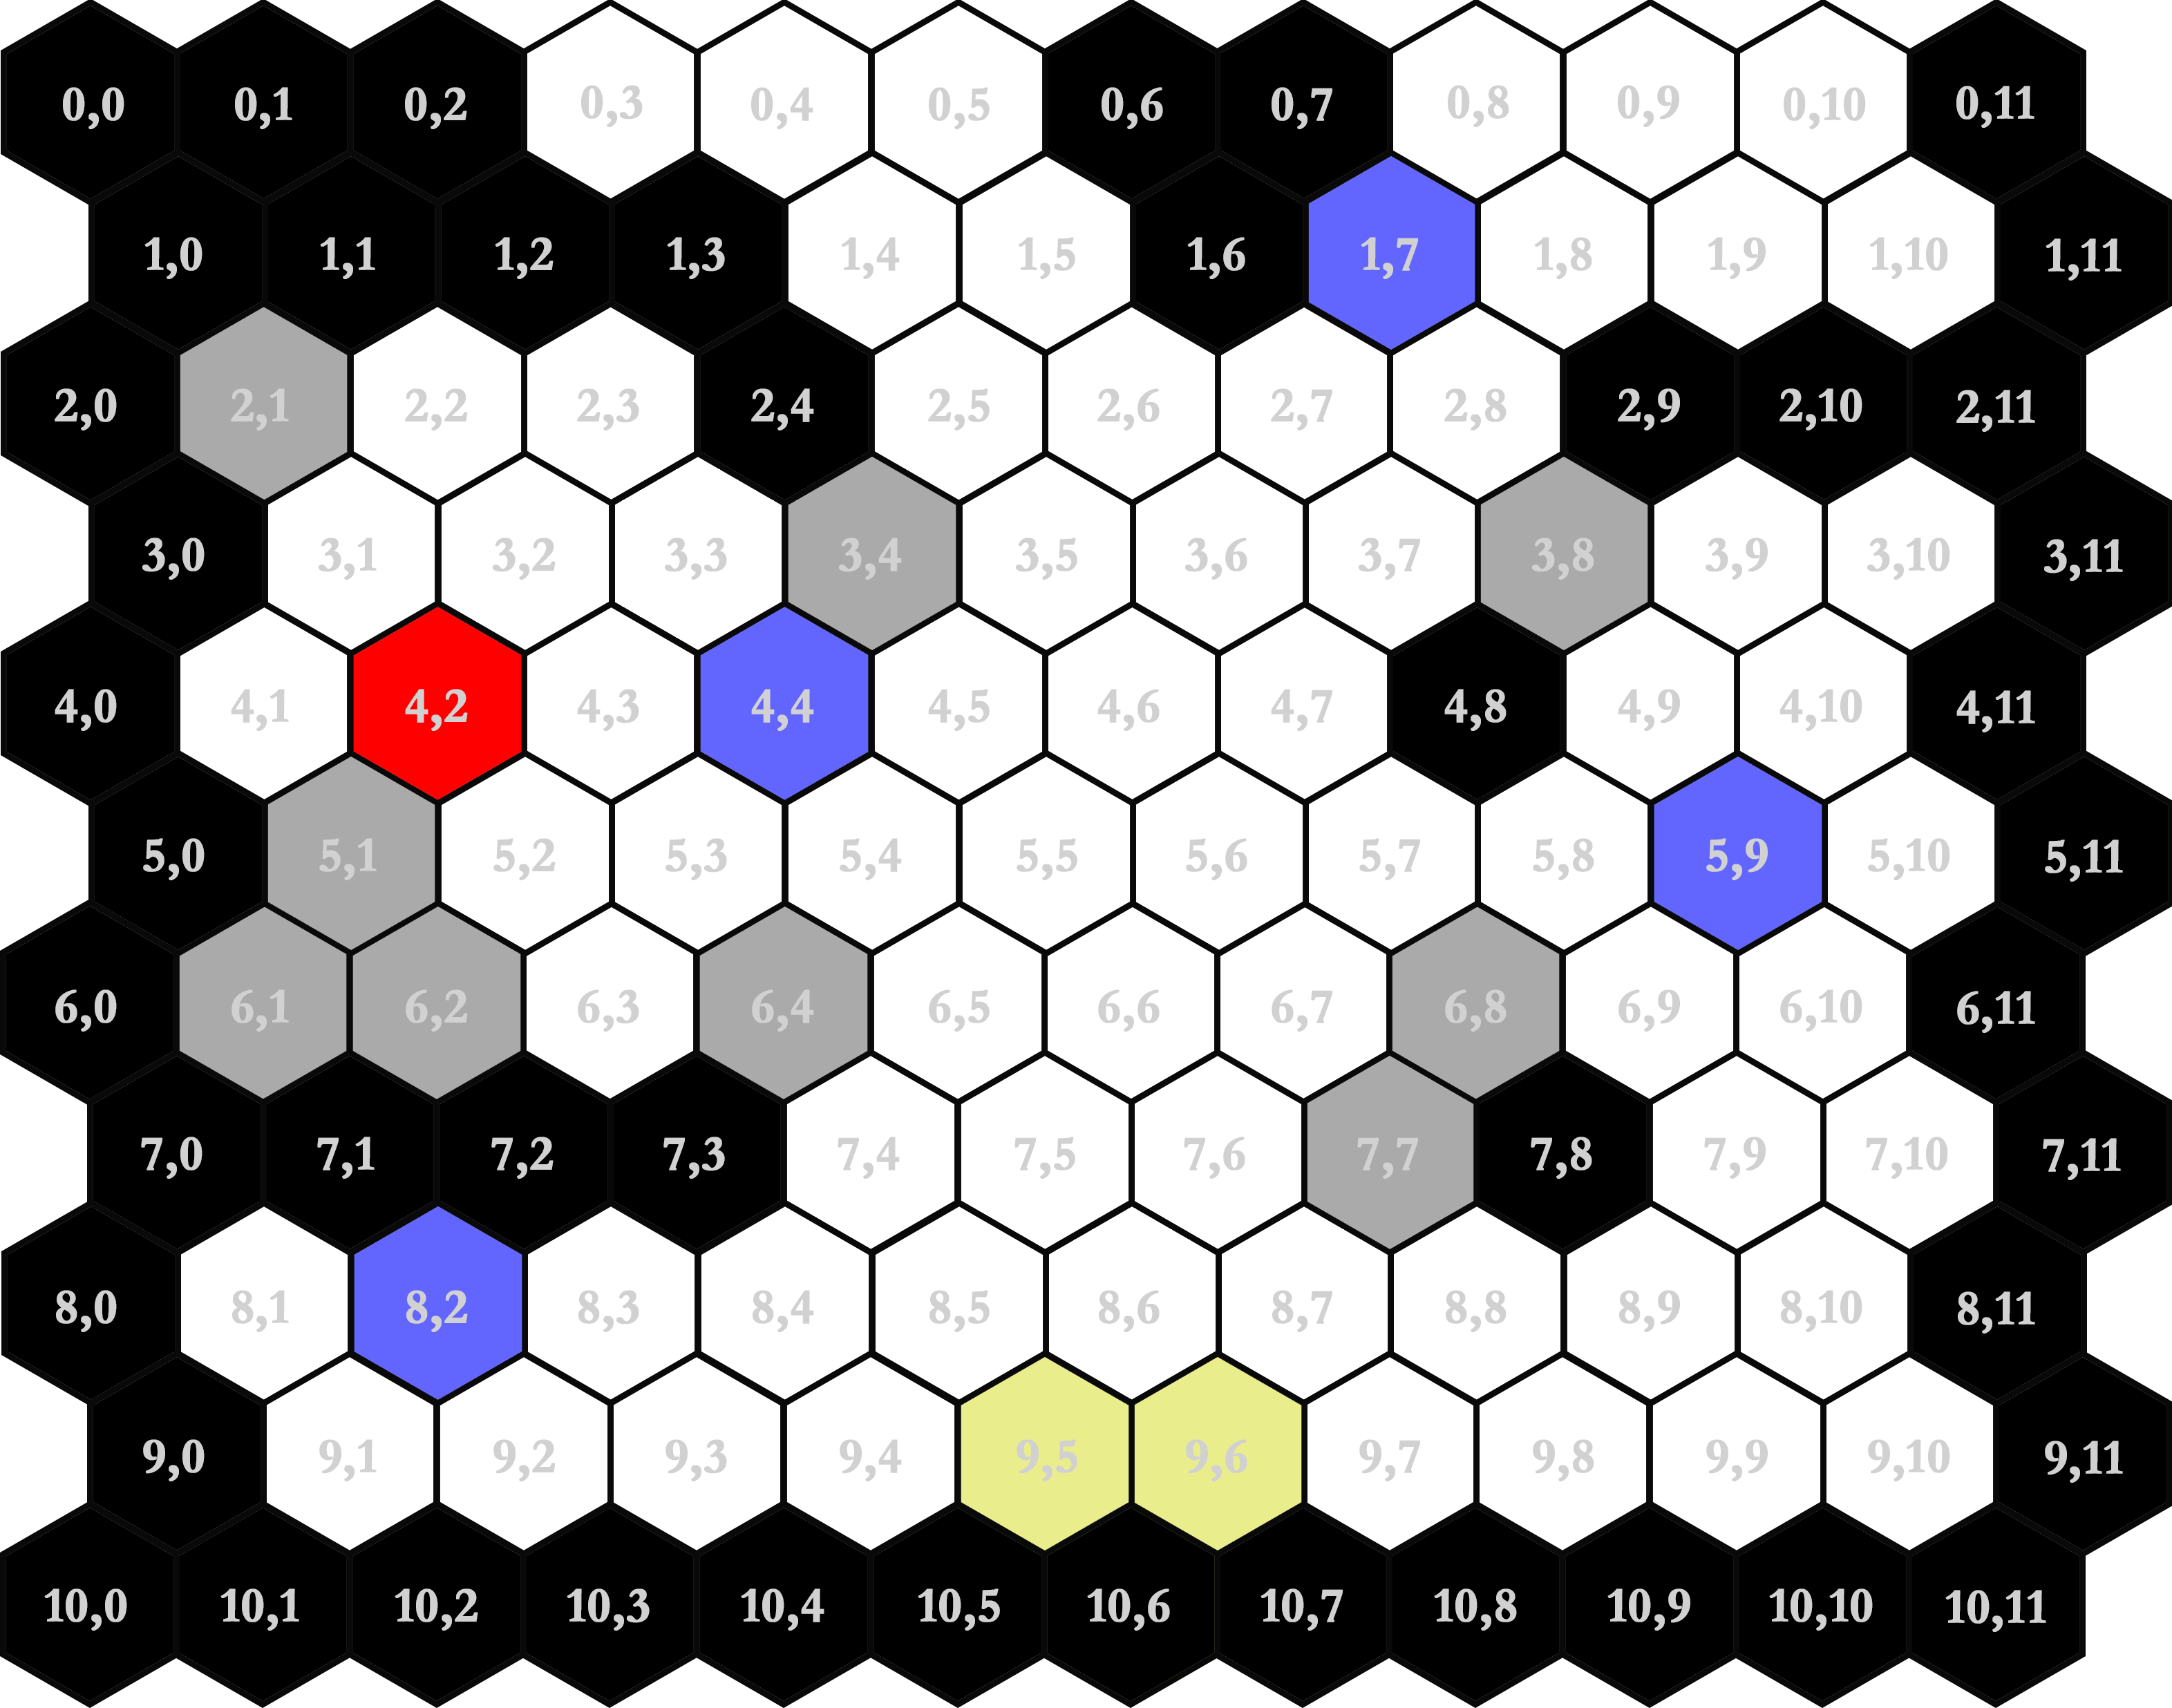
\includegraphics[width = 0.96\textwidth]{./maps/c317.png}
}
\end{center}

\subsection*{Setup Instructions}
\begin{itemize}
\item \textbf{Goldenrod:} Character Start Location. Place the character on either tile.
\item \textbf{Red:} Enemy Start Location. Place Zealot Eóghainn on this tile.
\item \textbf{Blue:} Enemy Start Location. Place a Risen Prisoner on \emph{two} of these tiles.
\item \textbf{Black:} Impassable Boundary/Full-Cover
\item \textbf{Light Gray:} Half-Cover.
\end{itemize}

\pagebreak

\subsection*{Victory}
The man stumbles backwards a few steps, then drops to a knee and clutches his side.\\

“Very well.”\\

He gasps and pants.\\
“By King Z*l. Ye have... \emph{haa}... rightfully reassumed the mold that begotten ye. \emph{Haa}... \emph{haa}...”\\

He rakes a forearm across his brow, plastering its arm hairs against the skin, then stands.\\

\notegain{c317a} Zealot Eóghainn has assessed His champion\\
>> \turnto{c317x1}

\subsection*{Defeat}
You lay in defeat. A trio of risen corpses shambles towards you with grasping hands. Then the man raises his arms, and they collapse in place--like marionettes cut from their strings.\\

“A valiant attempt. But just an attempt, nonetheless.”\\

The man approaches you with a hand outstretched, and lifts you onto your feet.\\

\notegain{c317b} Zealot Eóghainn has assessed His champion\\
>> \turnto{c317x1}